This chapter outlines the details behind some of the implementation choices in \dipter{}, specifically related to GLSL shader composition and code reuse in section \ref{sec:ImplementationProceduralShadingGLSL}, and how PyTorch shaders were implemented to mimic the GLSL shaders in section \ref{sec:ImplementationPyTorchShader}. Finally, some useful details behind the OpenGL rendering pipeline are presented.

\section{GLSL Shader} \label{sec:ImplementationProceduralShadingGLSL}
 As in many other programming languages, a fragment shader written in GLSL needs a main function as an entry point of execution. However, to simplify shader composition, all shaders in DiPTeR are defined as a single function (but may call other functions), with one exception; the \textit{material output shader}, which contains the only \texttt{main} function and must therefore always be the root node in any procedural texture. The different types of shaders in the OpenGL graphics pipeline, see section \ref{sec:OpenGLRenderingPipeline}, are all assembled into a \textit{Program} whose inputs are controlled via parameters called \textit{uniforms}. Each time a new node is connected to the node graph, all the needed code is assembled into one file by our GLSL code parser, where each unconnected parameter of each shader node in the graph is controlled via a uniform. These uniforms, much like any function parameters, need to have unique names which can be partly solved by appending the name of the shader function to the parameter name. However, while the parser ensures that needed function definitions are only inserted once, there are no guarantees that the names of the functions are unique. A modified function name is therefore constructed by also appending the name of the containing source file to the function name and because all shaders are defined in the same folder, this guarantees a unique function name. However, in the case where multiple shader nodes of the same kind are used in a node graph, this is not enough to guarantee a unique uniform name. A \texttt{Material} class is used to add nodes to the node graph as well as assigning a number to each node that is unique among nodes of the same kind. This number is passed to the GLSL code parser responsible for generating the assembled GLSL code and uniforms can now be uniquely named by following the format \texttt{<unique function name>\_<node number>\_<parameter name>}. 
 

\subsection{\texttt{\#import} Preprocessor Directive}\label{sec:ImportPreprocessorDirective}

OpenGL has a number of so called \textit{preprocessor directives}, operators that are processed before shader compilation and are called using the pattern \texttt{\#<directive-name> <arguments>}. None of these allow the user to import and reuse code from other files and while that is not a vital function for our project, it is certainly very helpful. Consequently, we implemented our own preprocessor directive called \texttt{\#import} which takes the name of a file to import as an argument. This directive is then parsed by our GLSL parser and the needed files are appended to the code to be compiled. This allows us to call functions from other files as if they were a part of the importing file's definition. 

\section{PyTorch Shader}\label{sec:ImplementationPyTorchShader}

As explained in section \ref{sec:MethodMatrixImplementation}, instead of implementing shading as a process that iteratively renders a texture pixel by pixel, we implement rendering as a function of matrices and render the image all at once. This means that a parameter in GLSL of type \texttt{vec3}, a vector of length 3, corresponds to a \texttt{Tensor} of shape $(W,H,3)$ in Python, where $W$ and $H$ are the width and height of the texture being rendered and the last dimension matches the GLSL parameter type. Unfortunately this implementation is a necessity due to lack of rendering support in PyTorch. While such a solution is immensely faster, it comes with some drawbacks in readability that can be mostly fixed with a few tricks that we will describe below, but also a serious lack of support for some important functionality pertaining to control flow in GLSL. Under the hood, all unconnected shader inputs are handled as scalars or vectors and are dynamically converted to matrix form just before rendering, while connected inputs are fetched by rendering from the connected node. 

Ultimately, measuring and confirming the correspondence between the GLSL and PyTorch implementations is done by explicitly measuring the difference between the two frameworks' renders for a variety of parameter combinations. However, it will greatly help the developer to correctly implement shaders in Python if the two languages can utilize similar syntax and call the same functions. To achieve this, we first have to implement parts of the GLSL standard library using PyTorch functions. This can be fairly tricky as the actual GLSL source code is not publicly accessible and may differ between GPU vendors, but some functions have a direct equivalent already implemented in PyTorch, or the mathematical formula for a given function may be revealed by the GLSL documentation. Furthermore, the use of some functions like the \texttt{step} function is problematic as it is not inherently differentiable. In this case we can implement the functionality using the PyTorch \texttt{sign} function, which is not strictly differentiable either, but can be backpropagated. Note that this and all other PyTorch functions support both scalars, vectors and matrices as all operations used are applied element-wise.


%\begin{minted}{python}
%def step(edge: Union[float, Tensor], x: Tensor) -> Tensor:
%"""
%`step` generates a step function by comparing x to edge.
%For element i of the return value, 0.0 is returned if x[i] < edge[i], 
%and 1.0 is returned otherwise.
%"""
%return (torch.sign(x-edge) + 1) / 2
%\end{minted}



Next, we demonstrate how the usage of vectors in GLSL can be translated to PyTorch. It is possible to extend the \texttt{Tensor} class in Python, one for each of the vector types in GLSL so that new vectors can be created by for example calling \texttt{vec3(...)}, but this is difficult as the implementation in PyTorch is convoluted, and we do not want to risk breaking the differentiability and portability. Instead, we create a library \texttt{vec.py} to handle the creation of vectors (or tensors), as well as supporting GLSL's syntax of retrieving elements of a vector by calling \texttt{var.x}, \texttt{var.y}, \texttt{var.z} or \texttt{var.w} as well as creating new vectors. In Code \ref{code:HSVGLSL} the GLSL implementation of our HSV shader is shown and in Code \ref{code:HSVPyTorch} the equivalent PyTorch implementation is shown. By implementing the GLSL standard library and the \texttt{vec} library, the implementations can be kept almost identical.

\begin{codefig}
\begin{minted}{glsl}
vec3 hsv(vec3 frag_pos, float h, float s, float v) {
    vec3 c = vec3(h,s,v);
    vec4 K = vec4(1.0, 2.0 / 3.0, 1.0 / 3.0, 3.0);
    vec3 p = abs(fract(c.xxx + K.xyz) * 6.0 - K.www);
    return c.z * mix(K.xxx, clamp(p - K.xxx, 0.0, 1.0), c.y);
}
\end{minted}
\caption{GLSL implementation of the HSV shader function.}
\label{code:HSVGLSL}
\end{codefig}

\begin{codefig}
\begin{minted}{python}
# Import standard GLSL library as 'gl' and vector library 'vec'
from dipter.shaders.lib import glsl_builtins as gl, vec  
def shade_mat(self, h: Tensor, s: Tensor, v: Tensor) -> Tensor:
    c = vec.vec3(h,s,v)
    K = vec.vec4(1.0, 2.0 / 3.0, 1.0 / 3.0, 3.0)
    p = torch.abs(gl.fract(vec.xxx(c) + vec.xyz(K)) * 6.0 - vec.www(K))
    return vec.z(c) * \
        gl.mix(vec.xxx(K), torch.clamp(p - vec.xxx(K), 0.0, 1.0), vec.y(c))
\end{minted}
\caption{PyTorch implementation of the HSV shader function, equivalent to the GLSL implementation in Code \ref{code:HSVGLSL}.}
\label{code:HSVPyTorch}
\end{codefig}

GLSL supports the basic control statements that we are used to in programming like \texttt{while}, \texttt{for} and \texttt{if} statements. One of the flaws with using matrices as parameters becomes obvious if we try to use them in the condition of any Python control flow. To substritute \texttt{if} statements, the PyTorch function \texttt{where} can be used which can evaluate a condition on each position in our matrix, and return a specific value at each position that evaluates to true or another value where it evaluates to false and the only drawback is breaking the syntax conformity. Unfortunately, there is no equivalent function for loops which means we are unable to handle the case where the loop counter is passed from a function argument.

There are a few other discrepancies that need to be managed. Firstly, while a shader in GLSL can utilize a number of different data types such as integers and booleans, the use of such datatypes will break differentiability in PyTorch and we will therefore always work with 32-bit floating point data. In practice however, we can support the use of parameters of any datatype in PyTorch as long as we do not let them be connectable, that is, prohibit the user from connecting such inputs to other nodes. This means that the value of such a parameter must be manually set by the user and are never converted to matrix form. This is utilized, for example, in our \textit{math shader} which returns the result of applying a selected mathematical operator to two values. The mathematical operator, \texttt{+}, \texttt{-}, \texttt{/} or \texttt{*} is selected by comparing the value of an input scalar integer, marked unconnectable and therefore not converted to matrix form, using \texttt{if} statements. The same workaround can be used to address the problem of letting the user control a loop counter, with the only drawback that it will be uniform across the entire texture. Secondly, most implementations of OpenGL supports division by zero, or must at least not lead to an interruption, which differs from Python where division by zero leads to a runtime exception. To remedy this, we add a small float constant to the denominator of all division operations in Python. Finally, the use of bitwise operators are common in GLSL but are only supported for integer types. This is also true for PyTorch, but as integer types are not differentiable the use of bitwise operators in \dipter{} is not possible. Fortunately, it is almost always possible to rewrite code without these operators, possibly at the expense of performance.

% \subsection{Shader Composition}

% \begin{enumerate}
%     \item How is it done in python, how are Tensors tracked and returned so that the same reference is always returned for \texttt{render()}, otherwise backprop will not work...
%     \item Explain that this is possible due to PyTorch only tracking torch operations done on it.
%     \item frag\_pos is calculated once in shader super class...
% \end{enumerate}

% \textbf{Cut from Stochastic Gradient Descent in Background...}
% As seen in the algorithm pseudocode and briefly explained in \ref{sec:ComputationalGraph}, we don't actually need the loss to take the set of parameters as input, thanks to the way \textit{PyTorch} registers operations done on any tensor in the set $\theta$ separately for each parameter. 


\section{Tools}

\subsection{OpenGL Rendering Pipeline}\label{sec:OpenGLRenderingPipeline}

\begin{figure}[!h]
    \centering
    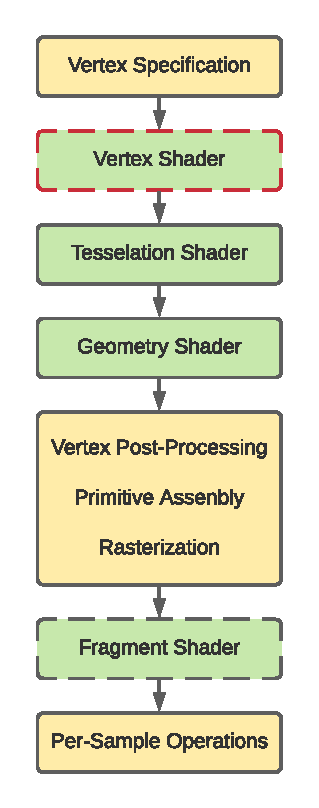
\includegraphics{img/implementation/RenderingPipeline2.pdf}
    \caption{An overview of the different stages in the OpenGL Rendering Pipeline. The stages marked green are programmable by user-defined shaders and the yellow stages are controllable through OpenGL function calls. The Vertex Shader, outlined in red, is the only shader that is required to be defined by the user. Lastly, a dashed outline marks the only two stages that are used in this project.}
    \label{fig:RenderingPipeline}
\end{figure}


The OpenGL rendering pipeline consists of multiple different stages that define a workflow, starting with 3D vertex data to finally producing 2D pixels on a screen \cite{a2019_rendering}. Some of these stages are programmable by the user, marked in green in Figure \ref{fig:RenderingPipeline}, where the Vertex Shader is the only one \textit{required} to be defined by the user. In the Vertex Specification step, no shader is used, but a list of vertex positions is defined to be rendered as well as a list of triangles that define the faces between these vertices. The Vertex Shader is run on each of these vertices and takes exactly one vertex as input and outputs exactly one vertex. This shader typically also takes three transformation matrices as input that define the scaling, translation and rotation of the object. These are used to output vertices in \textit{clip space} where coordinates are normalized to the interval $[-1,1]$. Next up is the Tesselation Shader and the Geometry Shader. Both manipulate or create geometry but neither are used in our project, as we are only interested in the look of the objects texture, not its geometry. Before the Fragment Shader stage, there is a crucial \textit{rasterization} stage that needs to be completed. This stage turns primitives (like triangles) into fragments, by looping over screen pixels and checking if they lie inside the boundaries of a primitive. If they do, a fragment is created for this pixel and the fragment is given per-vertex values that are interpolated between the vertices that make up the primitive, see section \ref{sec:Interpolation}. The fragments are closely related to screen pixels, but contain more information and each pixel can spawn more than one fragment, depending on multisampling parameters. Each fragment is then sent, one by one, to a Fragment Shader (also called Pixel Shader) which is where all the computations are done that define the final color of a single fragment. In essence, a fragment shader defines a function $f(V,P) \mapsto (r,g,b,a)$ that takes a set of interpolated per-vertex parameters $V$ and a set of user defined parameters $P$ as input, and outputs a fragment color on the form $(r,g,b,a)$, where $r$, $g$, $b$ are the value of the red,green and blue channels respectively and $a$ is the alpha value of the fragment.

% \subsubsection{Coordinate Systems}\label{sec:CoordinateSystem}

% \textbf{IMAGE EXPLAINING THE DIFFERENT SPACES!} \href{https://learnopengl.com/Getting-started/Coordinate-Systems}{SOURCE}

% In OpenGL there are five different coordinate spaces of interest, and three different transformation matrices that are used to convert between them. The first, \textit{object space}, is the space that is local to a 3D object in the scene. The axes of the local object space are static in relation to the object, no matter how the object is rotated, translated or scaled. As a comparison, a persons left and right will always be the same in relation to that person, but different when compared to another person because it is local to that person. To be able to position object relative to each other, we define a world space. Again, using a real world comparison, this corresponds to the cardinal directions of earth. Moving two objects north on global space, even with different individual local rotations, would move them along the global y-axis. To convert object coordinates to global coordinates, they are multiplied with a matrix often referred to as the \textit{object-to-world} matrix. In OpenGL, we do not need to render everything in the 3D scene, but only what is seen from a camera or viewer's point of view. As such, this space is referred to as view space or camera space. Coordinates in world space are converted to view space with a matrix conveniently referred to as the \textit{world-to-view} matrix. The object are now in a coordinate space that makes sense to the user. Moving an object left to right in view space (along x-axis) will move it left to right on the screen. However, as an OpenGL convention, any vertices outside of the range $[-1,1]$ will be \textit{clipped} or discarded and thus not rendered. Therefore, the next space is referred to as clip space and the coordinates in the range $[-1,1]$ as \textit{Normalized Device Coordinates} or NDC. A user can either define all of its vertices as NDC or in an arbitrary coordinate system and normalize them at this stage. The coordinates are converted from world space to clip space using a \textit{view-to-projection} matrix as the process of converting user defined coordinates to NDC (that are easy to map to a two dimensional coordinate system) is called \textit{projection}. This matrix comes in two forms, depending if \textit{perspective} or \textit{orthographic} projection is used.

% Using the three matrices, it's straight forward to attain the final NDCs in clip space by multiplying the vertices in user defined coordinates with each matrix as seen in equation \ref{eq:ObjectToClipCoordinates}. This defines the required output of the vertex shader, but there is one last important coordinate space to be aware of. This process is called the \textit{viewport transform} and converts the NDCs to screen coordinates, so that each point is mapped to a pixel on the screen. This coordinate system has its origin in the lower left corner of the screen at position $(0,0)$ and runs up to the defined resolution for the OpenGL viewport \textbf{IMAGE SHOWING THIS?}.

% \begin{equation}\label{eq:ObjectToClipCoordinates}
%     V_{clip} = M_{view-to-projection} \cdot M_{world-to-view} \cdot M_{object-to-view} \cdot V_{user}
% \end{equation}
